\documentclass[12pt]{article}
\usepackage{graphicx}
\usepackage{xspace}
\usepackage{color, colortbl}
\usepackage{amssymb}
\usepackage{amsmath}
\usepackage{mathtools}
\pagestyle{empty}
\definecolor{Gray}{gray}{0.9}
\textwidth      165mm
\textheight     240mm
\topmargin      -18mm
\oddsidemargin  -2mm
\evensidemargin 2mm
\newcommand{\impl}{\mathbin{\Rightarrow}}
\newcommand{\biim}{\mathbin{\Leftrightarrow}}
\newcommand{\id}[1]{\mbox{\textit{#1}}}
\newcommand{\ma}{\mathsf{a}}
\newcommand{\mb}{\mathsf{b}}
\newcommand{\mc}{\mathsf{c}}
\newcommand{\deriv}{\ensuremath{d_1}}
\renewcommand{\theenumi}{\alph{enumi}}

\DeclarePairedDelimiter\Floor\lfloor\rfloor
\DeclarePairedDelimiter\Ceil\lceil\rceil

\author{Emmanuel Macario - 831659}
\title{COMP30026 Models of Computation Assignment 2}
\date{October, 2018}

\begin{document}

\maketitle

% CHALLENGE 4
\subsection*{Challenge 4}

\begin{enumerate}
\item
Let $D$ be a DFA $(Q,\Sigma,\delta,q_0,F)$ that recognises regular language, $R$. We can transform 
$D$ into an NFA $N$ that recognises $\id{drop}(\ma,R)$ by replacing every transition that consumes input symbol
$\ma$ with an epsilon transition.

\bigskip
\noindent
More formally, we can define $N$ to be the five-tuple $N=(Q,\Sigma_\epsilon \setminus \{\ma\},\delta',q_0,F)$
with transition function,

\[
  \delta'(q, x) =
  \begin{cases}
  	\{\delta (q, x)\}     & \text{if $q \in Q$ and $x \in \Sigma \setminus \{\ma\}$} \\
      \{\delta (q, \ma)\} & \text{if $q \in Q$ and $x = \epsilon$} \\
  \end{cases}
\]

\bigskip
\noindent
Therefore, since $\id{drop}(\ma,R)$ can be recognised by NFA $N$, then $\id{drop}(\ma,R)$ is a regular language.
\bigskip

\item $L=\{a^m b^n c^n \mid m, n \geq 0\}$
\end{enumerate}
\bigskip


% CHALLENGE 5
\subsection*{Challenge 5}

Let $A$ be an arbitrary regular language. Since $A$ is regular, there exists some DFA $D$ that acts as a recogniser for $A$.

\bigskip
\noindent
We can systematically translate DFA $D=(Q,\Sigma,\delta,q_0,F)$ into a PDA $P=(Q',\Sigma',\Gamma,\delta',q'_0,F')$ with only three states, that recognises $A$.

\bigskip
\noindent
The general premise of this translation is to let the PDA use its stack to keep track
of the current state in the DFA, with respect to the previous input consumed. Additionally, 
we will only allow the PDA to accept an input string if the state on top of the stack is an original 
accept state in the DFA. The three state PDA can be seen as follows.

\begin{center}
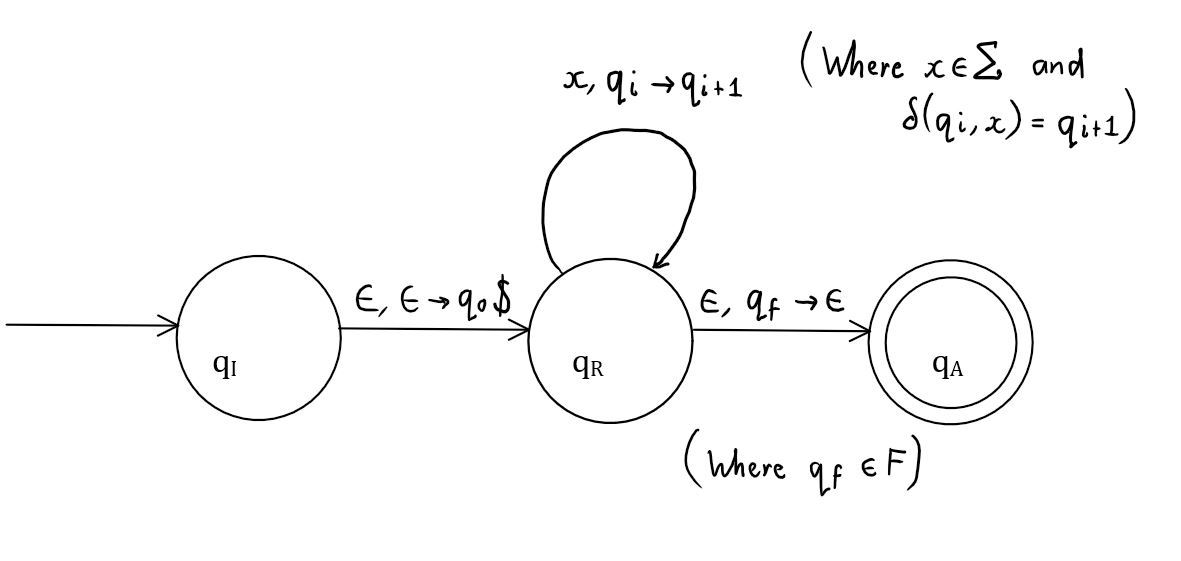
\includegraphics[width=5in,height=5in,keepaspectratio]{Q5-PDA.jpg}
\end{center}

\noindent
We can formally define P to be the six-tuple $P=(\{q_I, q_R, q_A\}, \Sigma, Q, \delta', q_I, \{q_A\}\}$
with transition function,

\[
  \delta'(q, x, s) =
  \begin{cases}
  	\{(q_R, q_0\$)\}   & \text{if $q=q_A$, $x=\epsilon$ and $s=\epsilon$} \\
      \{(q_R, q_n)\}        & \text{if $q=q_R$, $x \in \Sigma$ and $\delta (s, x)=q_n$} \\
      \{(q_A, \epsilon)\} & \text{if $q=q_R$, $x=\epsilon$ and $s \in F$} \\
  \end{cases}
\]
\bigskip

% CHALLENGE 6
\subsection*{Challenge 6}
We will show that $L(G) = A$ in two parts. Firstly, we will show $L(G) \subseteq A$ by using structural induction
on the form of $G$. Then, we will show $A \subseteq L(G)$ by induction on the length of strings in $A$.

\bigskip
\noindent
\textbf{Proof: $L(G) \subseteq A$}

\bigskip
\noindent
Let $w \in L(G)$ such that $S \impl^* w$. That is, let $w$ be an arbitrary string in $L(G)$ that is derived from 
start symbol, $S$. We will use structural induction to show that $w \in A$.

\bigskip
\noindent
Consider the base case $w = \epsilon$. Clearly, $w$ does not contain the substring 001.

\bigskip
\noindent
For the first recursive case, let $w=w'0$ where $w' \in L(G)$. By the inductive hypothesis, $w'$ does not contain
the substring 001. Hence, in this case $w$ cannot contain substring 001. This is because any new substrings generated 
will have 0 as the end symbol, whereas 001 has 1 as its end symbol.

\bigskip
\noindent
For the second recursive case, let $w=1w'$ where $w' \in L(G)$. By the inductive hypothesis, $w'$ does not contain
the substring 001. Hence, in this case $w$ cannot contain the substring 001. This is because any new substrings generated 
will have 1 as the start symbol, whereas 001 has 0 as its start symbol.

\bigskip
\noindent
For the final recursive case, let $w=01w'$ where $w' \in L(G)$. By the inductive hypothesis, $w'$ does not contain the
substring 001. Hence, in this case $w$ cannot contain the substring 001. This is because any newly generated substrings
of length three will be of the form $01x$ or $1xx$, where $x \in \Sigma_\epsilon$. Clearly, none of these substrings are equal to 001.

\bigskip
\noindent
Hence, in no case does $w$ contain substring 001. Therefore, $L(G) \subseteq A$.

\bigskip
\bigskip
\noindent
\textbf{Proof: $A \subseteq L(G)$}

\bigskip
\noindent
We would like to prove that for any binary string $s$ such that $s \in A, then s \in L(G)$. We can argue
the case using induction on the length of $s$.

\bigskip
\noindent
For the basis step, observe that any arbitrary string $s \in A$ for which $|s|=0$, $|s|=1$ or $|s|=2$, then $s \in L(G)$
is also true. This can trivially be seen for all possible strings in $A$ of length $\leq 2$ including $\epsilon$, 0, 1, 00, 01, 10 and 11.

\bigskip
\noindent
For the inductive step, assume that $k \geq 2$ and that all strings $s \in A$ of length $0$ to $k$ are included in $L(G)$.
Now, consider string $s' \in A$ of length $k+1$. If $s'$ ends with a 0, then $s' \in L(G)$ since the prefix of $s'$ of length $k$
is also in $L(G)$, by the inductive hypothesis. Similarly, if $s'$ starts with a 1, then $s' \in L(G)$ since the suffix of $s'$ of length
$k$ is also in $L(G)$. Finally, if $s'$ starts with 01, then $s \in L(G)$ since the suffix of $s'$ of length $k-1$ is also included in
$L(G)$, by the inductive hypothesis.

\bigskip
\noindent
Thus, we have shown that for any arbitrary length string $s$ such that $s \in A$, then $s \in L(G)$. It follows that $A \subseteq L(G)$.


\bigskip
\bigskip
\noindent
Since we have proven that both $L(G) \subseteq A$ and $A \subseteq L(G)$, it
follows that $L(G) = A$.


\end{document}